\section{Experiments as Claim Tests}
\label{sec:experiments}

Each experiment has one inferential role: verify the sharp boundary, show why
ideal membership is not a frequency heuristic, connect the diagnostic to a
learning-relevant instability, or test the representation hypothesis. The
primary axis is refinement at matched task and noise budgets, not isolated
single-resolution accuracy.

\subsection{The threshold predicts objective and estimator fluctuations}
\label{sec:exp-threshold}

We first use relative precision perturbations
$\lambda_j(H_N)=0.45j^{-\alpha}$ and increase the cutoff from $10$ to
$10^6$. The setting $\alpha=1.20$ exposes ordinary trace-class behavior;
$\alpha=0.60,0.50,0.40$ isolate the bounded, logarithmic, and polynomial
$\Schatten{2}$ regimes in \cref{cor:power-law}. The covariance map
$K_N=H_N(I-H_N)^{-1}$ from \cref{eq:precision-covariance-map} preserves these
regimes. At every finite cutoff, with $Z\sim\mathcal N(0,I)$, we verify
\begin{equation}
  \frac12\langle Z,H_NZ\rangle+\frac12\log\det(I-H_N)
  =\frac12\bigl(\langle Z,H_NZ\rangle-\operatorname{Tr}H_N\bigr)
   +\frac12\log\det\nolimits_2(I-H_N).
  \label{eq:finite-wick-identity}
\end{equation}
The two sides agree to numerical precision, while only the combined
Wick--$\det_2$ expression remains uniformly controlled in the
Hilbert--Schmidt, non-trace-class regime.
\Cref{fig:phase-boundary} shows the complete refinement path rather than a
single-cutoff snapshot.

The same panel tests the stochastic consequence using the matrix-free
objective. We hold the feature batch fixed and vary only its Rademacher probes.
Across a $64\times$ increase in dimension, the unfiltered branch increases
$\hsnorm{H_N}^2$ by $42.5\times$ and probe-induced gradient variance by
$102.7\times$; the Schatten-filtered branch changes by $1.21\times$ and
$1.46\times$,
respectively. This is an estimator-mechanism test, not a claim that $\Ttwo$
alone determines every source of SGD variance.

\subsection{Same frequency appearance, different continuum fate}
\label{sec:exp-matched-spectrum}

The decisive control constructs two perturbations that a spatial-frequency
heuristic cannot distinguish. Let $d=m^2$, let $0<\eta<1$, and let $U_d$ be a
flat DFT unitary in complex Fourier coordinates, so
$|(U_d)_{ij}|^2=1/d$ (a Walsh--Hadamard transform gives a real construction at
compatible $d$). Define
\begin{align}
  A_d^{\mathrm{stable}}
  &=U_d\operatorname{diag}\!\left(
    \eta,\underbrace{\tfrac{\eta}{m+1},\ldots,
    \tfrac{\eta}{m+1}}_{d-1}
  \right)U_d^\ast, \\
  A_d^{\mathrm{unstable}}
  &=U_d\operatorname{diag}\!\left(
    \underbrace{\eta,\ldots,\eta}_{m},
    \underbrace{0,\ldots,0}_{d-m}
  \right)U_d^\ast.
  \label{eq:matched-spectrum-pair}
\end{align}
They have exactly the same coordinatewise noise power, total noise power, and
leading-mode gain:
\begin{equation}
  \operatorname{diag}A_d^{\mathrm{stable}}
  =\operatorname{diag}A_d^{\mathrm{unstable}}
  =\frac{\eta}{m}\mathbf 1,
  \quad
  \operatorname{Tr}A_d^{(\cdot)}=\eta m,
  \quad
  \opnorm{A_d^{(\cdot)}}=\eta.
  \label{eq:matched-spectrum-observables}
\end{equation}
Their operator-ideal behavior is nevertheless opposite:
\begin{equation}
  \hsnorm{A_d^{\mathrm{stable}}}^2
  =\eta^2\frac{2m}{m+1}\longrightarrow2\eta^2,
  \qquad
  \hsnorm{A_d^{\mathrm{unstable}}}^2
  =\eta^2m=\eta^2\sqrt d\longrightarrow\infty.
  \label{eq:matched-spectrum-t2}
\end{equation}
We attach the same physical Fourier envelope to both families. Their radial
power spectrum, bandwidth, trace, operator norm, and low-frequency response
then remain matched, but their raw $\Ttwo$ and Gaussian objective fluctuations
separate with the rates in \cref{eq:matched-spectrum-t2}. A frequency-only
mask acts on the common envelope and cannot remove the unstable channel factor
without also sending the retained low-frequency response to zero. The main
comparison includes hard and smooth Fourier cutoffs, an unconstrained spectral
decay gate, and the ideal-aware gate at matched task distortion and noise
budget. Exact construction and matching constraints are in
\cref{app:frequency-controls}.

\begin{figure}[t]
  \centering
  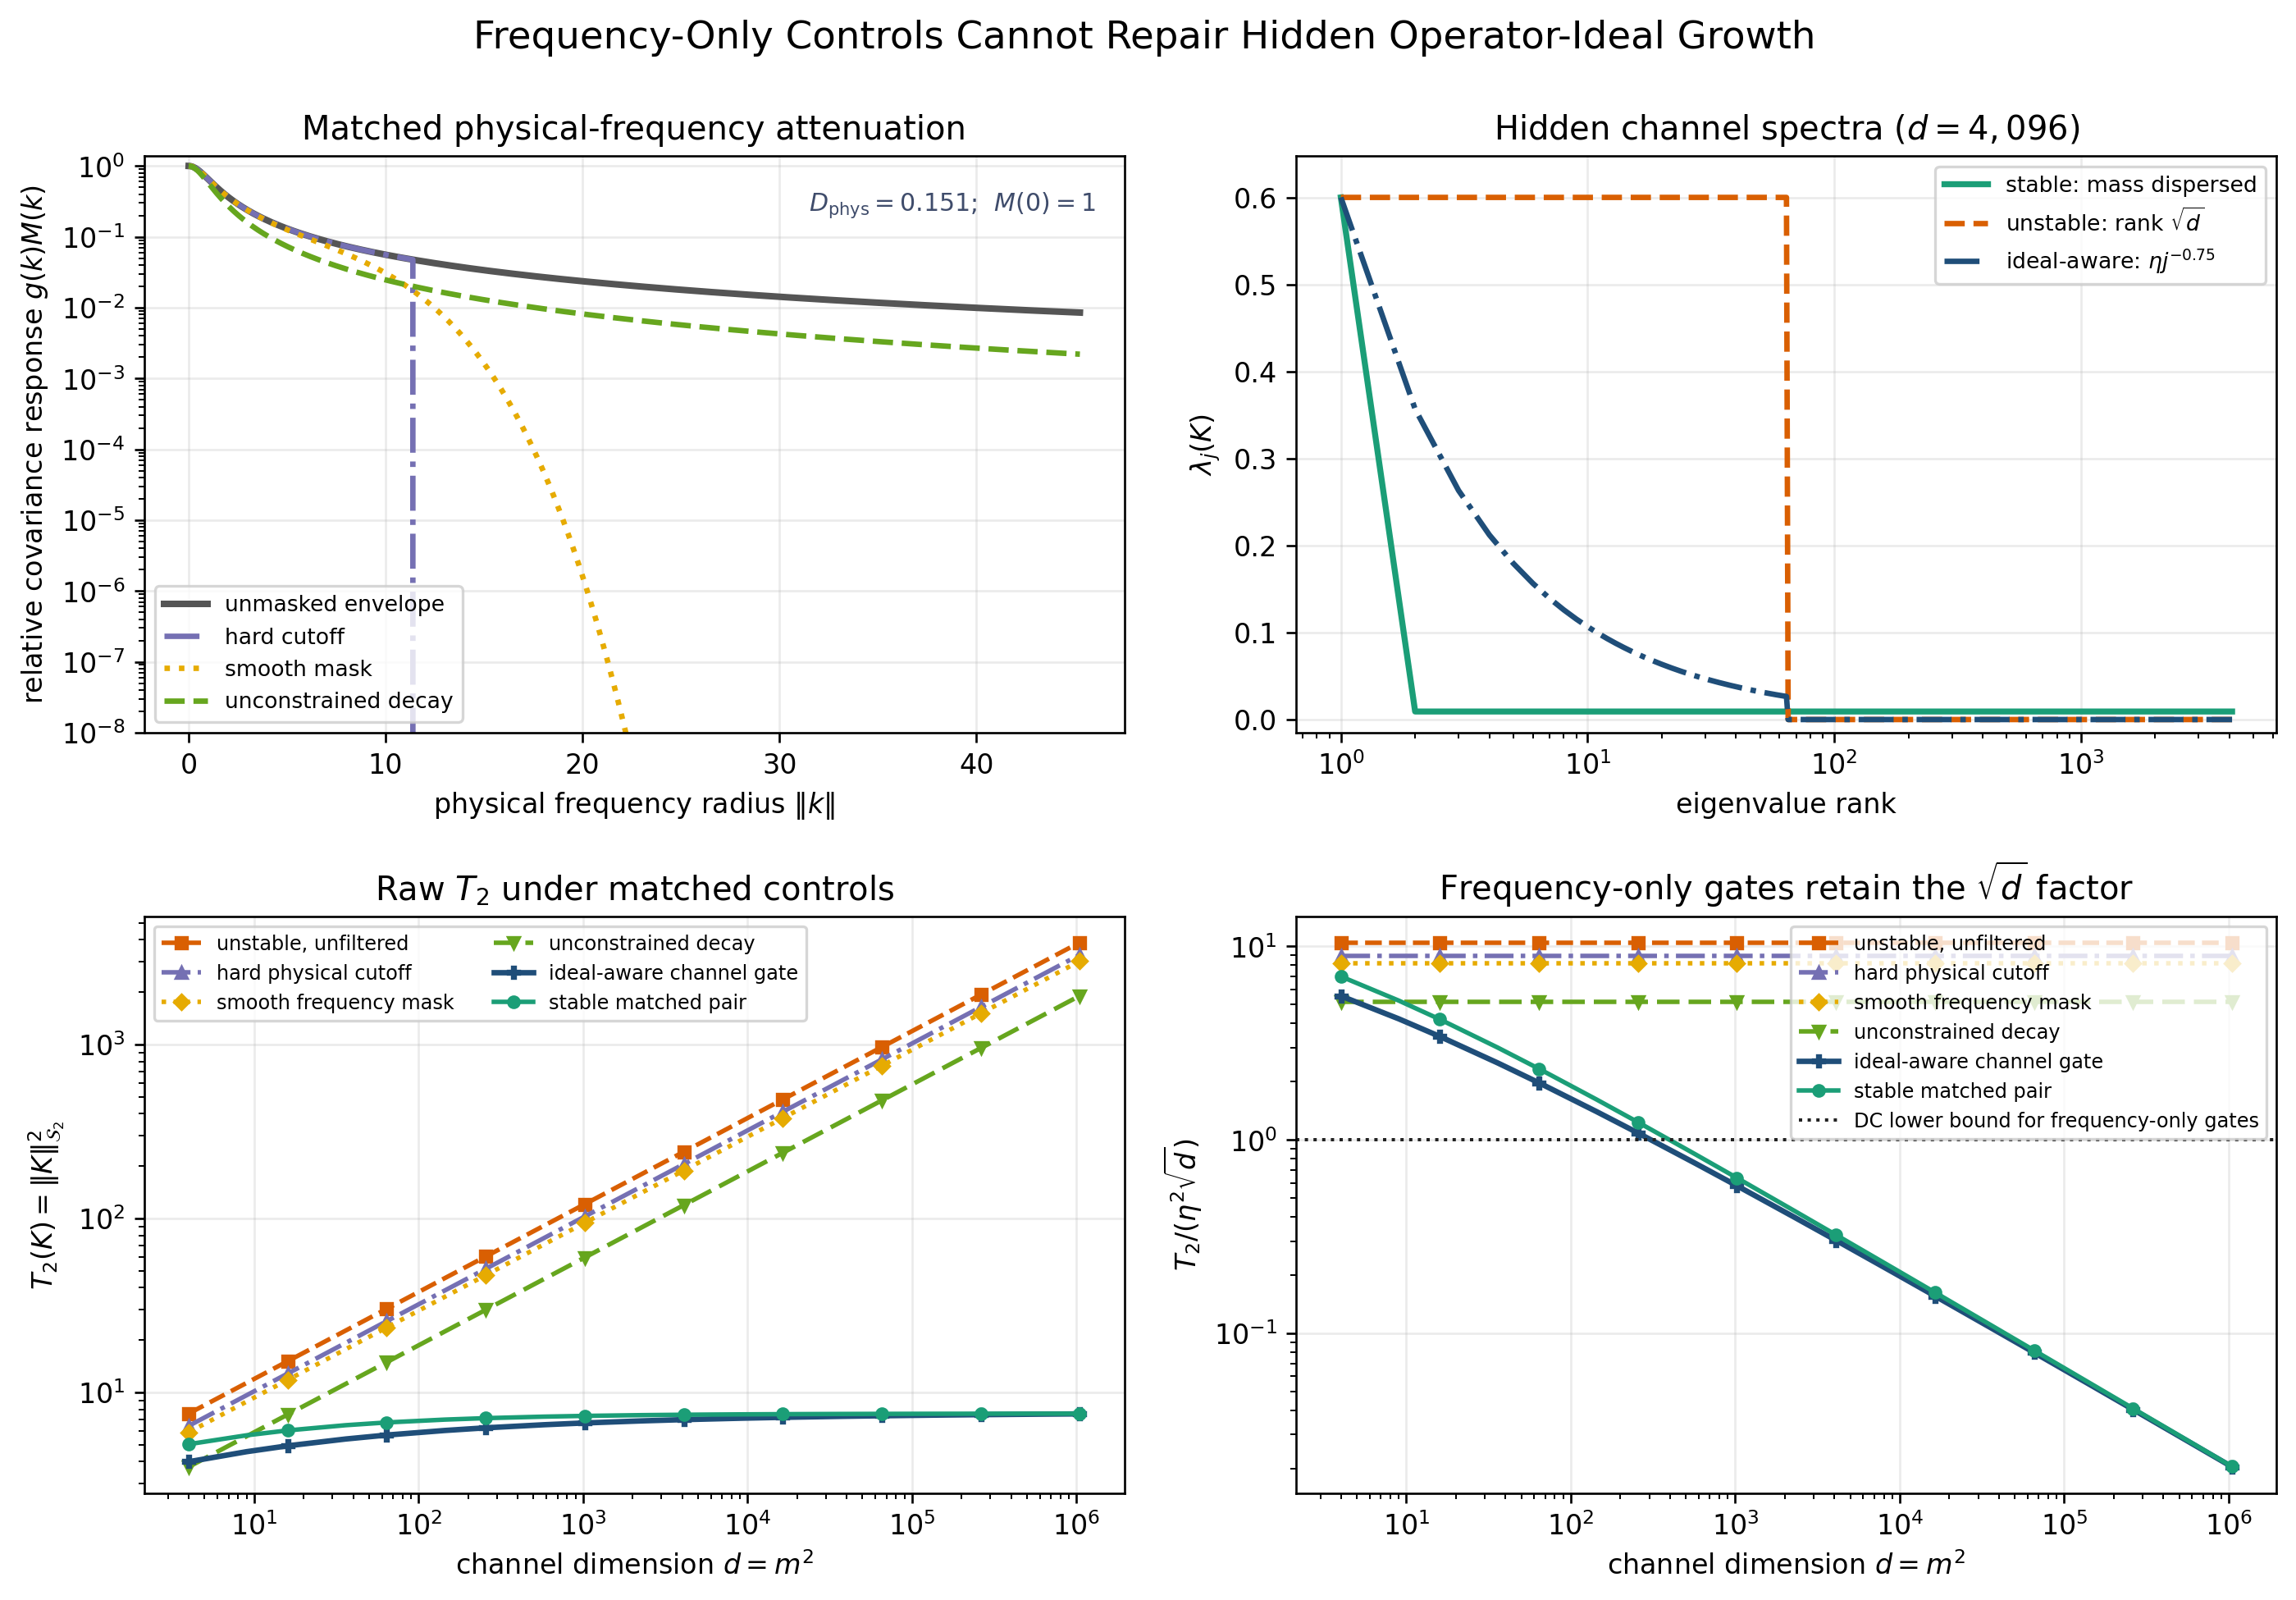
\includegraphics[width=\linewidth]{../experiments/toy/frequency_matched_schatten.png}
  \caption{\textbf{Frequency matching does not control operator-ideal
  accumulation.} The two families have identical radial Fourier diagonals,
  trace, and operator norm, but different hidden eigenvalue multiplicities. At
  $d=1{,}048{,}576$, the stable family has $\Ttwo=0.7193$, while the unstable
  family reaches $368.64$, a $512.5\times$ separation inherited by the exact
  Gaussian residue and centered quadratic variance. All curves are closed-form;
  explicit DFT matrices verify the identities at small $d$.}
  \label{fig:frequency-matched}
\end{figure}
\FloatBarrier

\subsection{Resolution-consistent operator learning}
\label{sec:exp-operator}

We discretize the same underlying continuous random fields on a resolution
ladder and train a neural operator at a base grid. The ideal-aware gate is
defined in physical Fourier modes,
\begin{equation}
  \beta_\theta(k)
  =\rho\operatorname{sigmoid}(a_\theta(k))
   (1+\lVert k\rVert^2)^{-s/2},
  \qquad
  s=1+\epsilon+\operatorname{softplus}(\gamma),
  \label{eq:physical-s2-gate}
\end{equation}
where $0<\rho<1$ and $\epsilon>0$ are fixed. Thus $s>1$ enforces square
summability in two spatial dimensions and keeps the series estimator inside
its spectral-radius domain. Here $\beta_\theta(k)$ is a relative covariance
eigenvalue, not a noise standard deviation. We freeze
the selected gate and evaluate zero-shot at $2\times$ and $4\times$ the
training resolution. Architecture, optimization steps, low-frequency
response, and base-resolution noise budget are held fixed.

Baselines comprise ordinary Gaussian noise, renormalization without filtering,
relative and fixed physical Fourier cutoffs, and an architecture-matched
smooth decay gate without the $s>1$ constraint. The primary outputs are raw
canonical $\Ttwo(R)$, minibatch-gradient variance, the drift of the independently
selected noise scale, zero-shot relative error, and the discretization defect
$\lVert D_R f_{2R}(U_Rx)-f_R(x)\rVert$. This experiment asks whether crossing
the theoretical threshold predicts a stable training intervention and
resolution transfer, beyond matched base-grid accuracy.

% Figure 3 and main table: raw-T2 growth, noise-scale drift, zero-shot transfer.

\subsection{Latent encoders expose an implicit filtering requirement}
\label{sec:exp-encoder}

We do not assume that compression automatically supplies operator-ideal
regularity. On an antialiased image-resolution ladder, we separately estimate
the encoder pushforward $K_{E,N}$ in \cref{eq:encoder-pushforward} and the
actual relative diffusion update $K_{\mathrm{diff},N,t}$ in
\cref{eq:diffusion-relative-covariance}. The controls are pixel identity, a
same-rank partial isometry, architecture-matched random encoders, antialiased
downsampling, a learned VAE encoder, and the learned encoder with an explicit
Schatten gate. The principal ladder allows latent spatial rank to grow with
resolution; fixed-rank bottlenecks are reported separately and are not treated
as evidence of nontrivial uniform $\Schatten{2}$ control.

The audit reports full covariance spectra, raw $\Ttwo(N)$ and its growth
exponent, effective rank, tail energy, and downstream noise-scale or gradient
drift. The latent reference covariance is estimated independently of the
injected perturbation, with a fixed support regularization rule across the
ladder. Raw $\Ttwo$ under the quadrature-weighted discretization inner product is the
membership test; normalized effective-rank summaries are complementary
descriptions, not substitutes. This experiment answers the representation
question directly: which encoders change the spectral class in which noise
acts, and when explicit filtering supplies what compression alone does not.

% Figure 4: encoder and diffusion-update spectra, raw-T2 growth, training consequence.
